\chapter{Теоретическое исследование и архитектура}\label{arch}

\tbd{Содержание главы}

\section{Поиск вероятностных лазеек}\label{arch:rbs:schema}

В данном разделе описаны алгоритмы поиска вероятностных лазеек.
Для поиска вероятностных лазеек применяются эволюционные алгоритмы, а именно, $(1 + 1)$ и $(\mu + \lambda)$
алгоритмы~\cite{bib:ea},~\cite{bib:ga}. Для полного описания теоретической схемы поиска
вероятностных лазеек необходимо определить особь, фитнес-функцию, а также операторы скрещивания,
мутации и отбора.

\textbf{Особью} во всех реализованных схемах поиска вероятностных лазеек является битовая маска
$\overline{B}$, соответствующая множеству переменных $B$, включенных в лазейку.

\textbf{Фитнес функция}. В фитнес-функции используется аппроксимация значения $\rho$, формально 
определенная уравнением \ref{overview:rho-hat}, так как такой
подход позволяет вычислять его с достаточно высокой точностью, а главное --- быстро. В качестве
алгоритма $A$ используется алгоритм вывода последствий (определение~\ref{overview:prop}), 
эффективно реализованный в рамках решателя Minisat~\cite{bib:minisat}. Данный алгоритм с точки 
зрения решателя не является полным, но имеет полиномиальное время работы.

Используется фитнес функция, описанная в \tbd{paper}. Её преимущество заключается в том, что она помимо
максимизации $\hat{\rho}$-значения лазейки минимизирует её размер. Максимизация $\hat{\rho}$-значения 
достигается первой частью функции:
\[
    G_{C}\left(\overline{B}\right) = (1 - \hat{\rho}_B) \cdot 2^{\omega |V|},
\]
где $C$ --- формула \ref{overview:formula}, $V$ --- множество переменных в формуле, $w \in (0, 1]$
-- константа. Минимизация размера лазейки обеспечивается второй частью функции:
\[
    f_{C, \min{|B|}} = \hat{\rho}_B \cdot 2^{|B|}.
\]
Действительно, при относительно близких значениях $\rho$ большое влияние на функцию будет оказывать
размер лазейки $B$. Итоговая фитнес функция выглядит следующим образом:
\begin{equation}
    f_{C}\left(\overline{B}\right) = \hat{\rho}_B \cdot 2^{|B|} + (1 - \hat{\rho}_B) \cdot 2^{\omega |V|}.
    \label{arch:fitness}
\end{equation}

\textbf{Операторы}
В качестве основного оператора мутации был выбран зарекоммендовавший себя в \tbd{paper} оператор
\textsc{Doerr}~\cite{bib:doerr}. В процессе разработки также использовался равномерный оператор
мутации, однако результаты, которые он показывал, стабильно хуже результатов \textsc{Doerr} на
всех примерах, поэтому он был отброшен, однако доступен в конфигурации. Реализованы операторы
одноточечного и двуточечного скрещивания. Генетический алгоритм $(\mu + \lambda)$ был
реализован аналогично схеме, предложенной в \tbd{paper}. Сравнение получившихся алгоритмов
проведено в разделе~\ref{research:evol}.

\section{Разбиение пространства поиска}\label{arch:split}

В данном разделе описан основной подход к разбиению задачи на подзадачи, а так же реализованные
подходы к использованию вероятностных лазеек в качестве опоры для разбиения задачи.

Для начала опишем общий подход к разделению задачи на подзадачи. Пусть есть формура $E$, 
содержащая переменные $V$. Зафиксируем подмножество переменных $B$. Тогда исходную
задачу можно разбить на подзадачи, соответствующие всем $2^{|B|}$ подстановкам переменных из $B$.
Решив каждую из этих подзадач, несложно сделать вывод и для исходной задачи:
\begin{itemize}
    \item Если хотя бы одна из подзадач оказалась выполнимой, то и исходная формула выполнима.
    \item Если все подзадачи оказались невыполнимыми, то и исходная формула невыполнима.
\end{itemize}

Именно таким способом в этой работе производится разбиение задач. Однако, в качестве множества
$B$ берется не случайное множество, а множество, так или иначе полученное через поиск вероятностных
лазеек, так как это, как будет показано данее, позволяет без непосредственного решения отсечь сразу
большую долю подзадач.

Опишем базовый подход, использующий одну лазейку. Пусть, как описано в
разделе~\ref{arch:rbs:schema}, найдена лазейка $B \subseteq V$. Тогда пространство поиска можно разделить
на $2^{|B|}$ подпространств, разделив тем самым задачу на $2^{|B|}$ независимых подзадач. Более 
того, хорошая вероятностная лазейка имеет аппроксимированное (а очень часто и точное) значение 
$\rho$ близкое к единице. Это позволяет сразу отсечь большую долю невыполнимых подзадач, используя 
только метод вывода последствий. Схема разделения пространства поиска содержится на 
рисунке~\ref{arch:split:filter}.

\begin{figure}[H]
    \caption{Схема разбиения пространства поиска на основе одной лазейки}
    \centering
    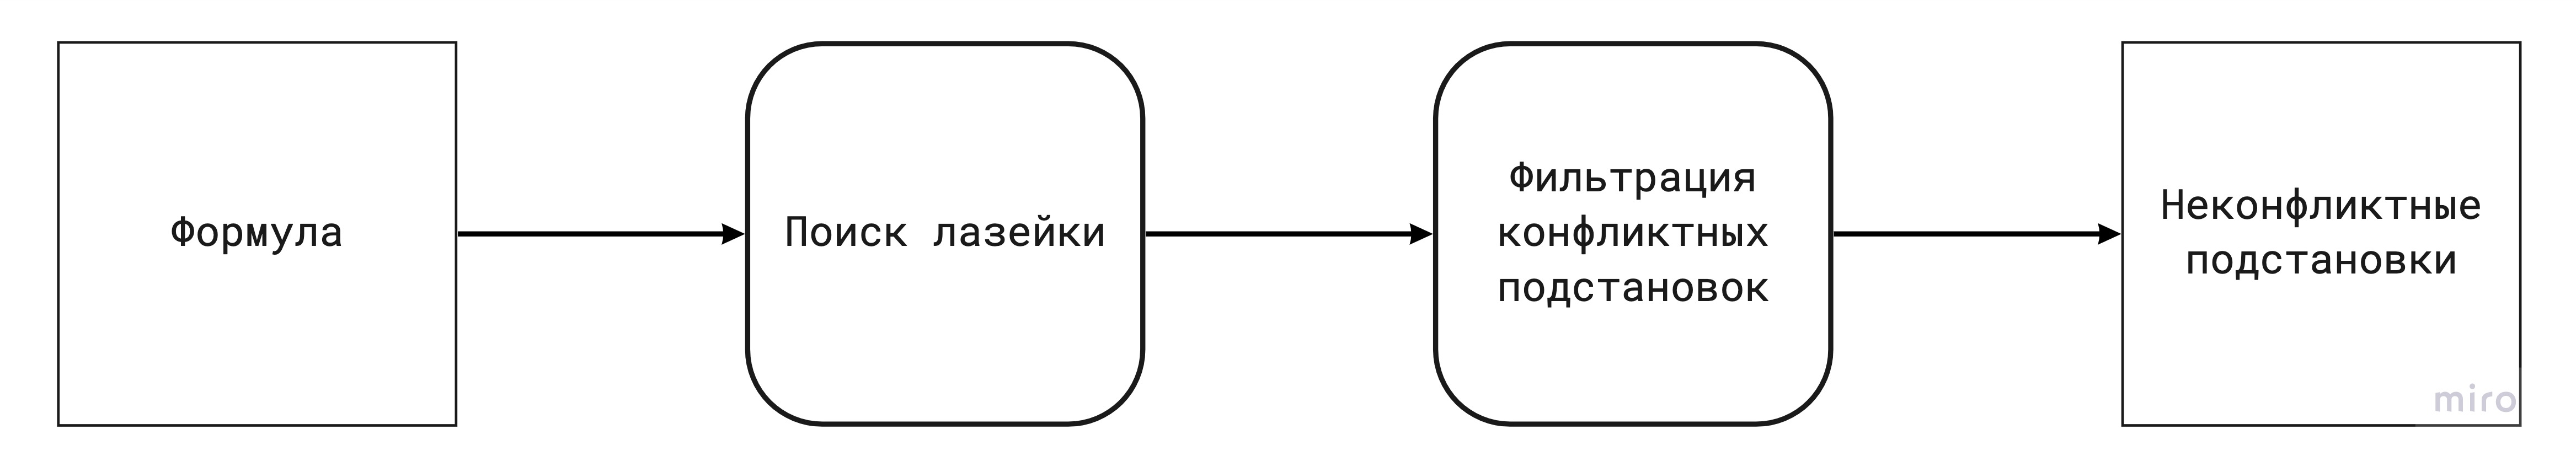
\includegraphics[width=\textwidth]{arch-filter}
    \label{arch:split:filter}
\end{figure}

Более продвинутый подход для разбиения пространства поиска, описанный в \tbd{paper}, устроен следующим
образом. Сначала находятся $K$ различных лазеек $\{\,B_i \subseteq V\,\}$. Далее для каждой лазейки 
независимо фильтруются подстановки, приводящие к конфликту. Множество неконфликтных подстановок,
полученных для лазейки $B_i$, обозначим за $C_i$. Далее формируется декартово произведение 
$\bigtimes_i\{C_i\}$, представляющее собой предварительное разбиение пространства поиска. Далее это
разбиение можно еще раз отфильтровать, избавившись от конфликтных подстановок.
Смысл данного подхода заключается в том, что объединение неконфликтных подстановок (а именно из
таких объединений состоит $\bigtimes_i\{C_i\}$) с немалой долей вероятности является конфликтной
подстановкой, так как содержит назначение для большего числа переменных. В исследованиях,
содержащихся в \tbd{paper}, данная догадка находит экспериментальное подтверждение, поэтому реализована
в рамках данной работы. Данная схема проиллюстрирована на рисунке~\ref{arch:split:cart}.

\begin{figure}[H]
    \caption{Схема разбиения пространства поиска на основе декартова произведения}
    \centering
    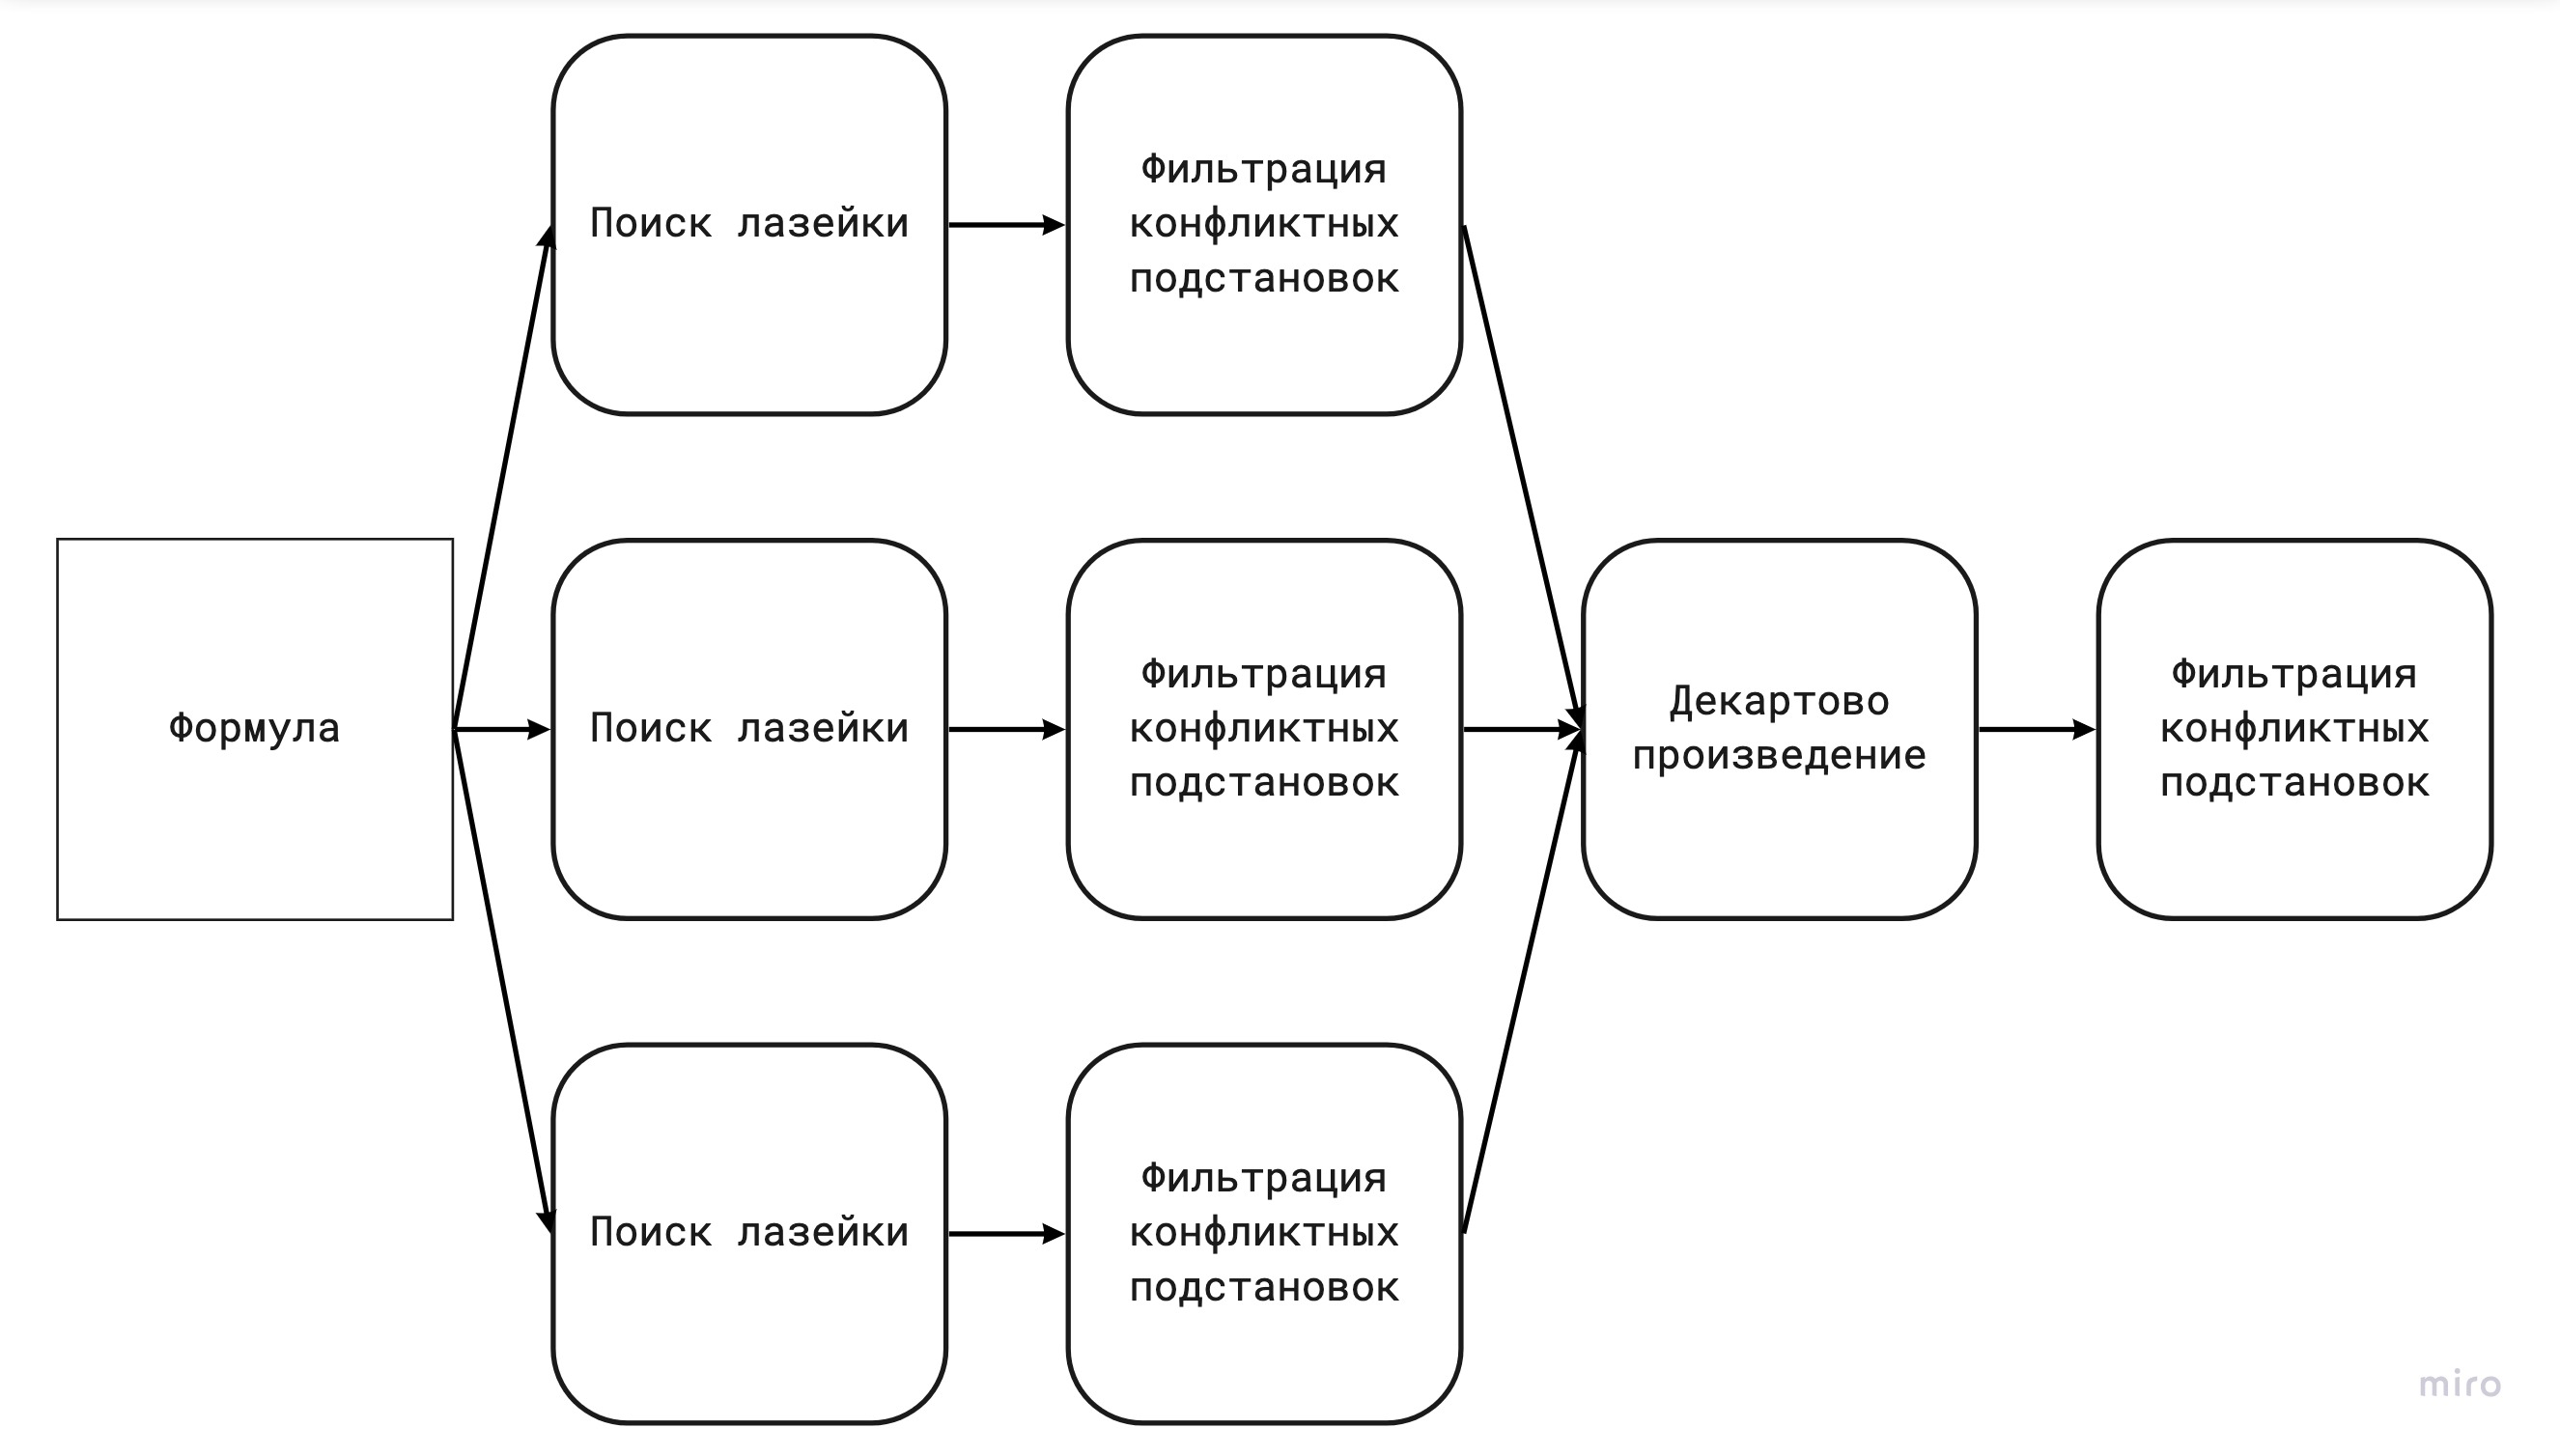
\includegraphics[width=\textwidth]{arch-cart}
    \label{arch:split:cart}
\end{figure}

Стоит обратить внимание на тот факт, что данная схема является более масштабируемой, нежели предыдущая,
так как искать различные лазейки можно параллельно, что и реализовано в данной работе. Сравнение
производительности данных схем проведено в разделе~\ref{research:final}.

\section{Схемы решения}\label{arch:solve}

В данном разделе описаны способы решения задачи булевой выполнимости на основе разбиений пространства
поиска, детально рассмотренных в разделе~\ref{arch:split}.

\textit{Прямое решение}. В данной схеме, аналогичной подходу, используемому в \paper{paper}, каждая
подстановка переменных $\hat{b}$, полученная в результате разбиения задачи на подзадачи, решается
каким-либо существующим решателем. В данной работе данный подход реализуется через сервис, описанный
в разделе~\ref{arch:solver}, что позволяет обеспечить параллельное решение с обменом знаниями между
решателями.

\textit{Рекурсивное решение}. Прямое решение имеет как минимум один критический для производительности
и масштабируемости недостаток. Он заключается в том факте, что очень часто сложность подзадач из
разбиения сильно варьируется. То есть, есть подзадачи, требующие большого количества ресурсов, главным
образом, времени, а есть подзадачи, решающиеся очень быстро. Для трудных подзадач разумной идеей
будет начать решение заново, то есть снова разбить подпространство поиска, соответствующее долго
решаемой подстановке $\hat{b}$ на подпространства таким же образом, как это сделано для исходной
задачи. Понятно, что такой подход можно продлить до любой глубины, однако осмысленно ограничить
количество переразбиений подпространств.

Опишем теперь более детально схему предлагаемого подхода. Определим стек задач, состоящий из
подстановок, подлежащих решению. Изначально этот стек состоит из одной пустой подстановки,
соответствующей исходной задаче. Далее, пока стек не пуст или не найдено решение, снимаем со стека
подстановку. Далее для данной подстановки, используя алгоритм, описанный в разделе~\ref{arch:split},
ищем разбиение на подзадачи. Для всех полученных подзадач запускаем решение, ограниченное по
времени. Ограничение по времени может зависеть от глубины рекурсии, а так же может быть бесконечным,
когда глубина рекурсии уже достаточно большая. Те подзадачи, которые не удалось решить за 
отведенное время, считаем трудными и кладем в стек для дальнейшего переразбиения и перерешивания.

Сравнение производительности подходов к решению подзадач описано в разделе~\ref{research:final}.

\section{Эффективный вывод последствий}\label{arch:rbs:prop}

Основным потребителем ресурсов в описанной схеме поиска вероятностных лазеек является алгоритм
вывода последствий, реализованный в Minisat~\cite{bib:minisat}. Поэтому оптимизация этого алгоритма
и разработка новых подходов является крайне важной задачей для достижения высокой производительности.

\textit{Выборка}\label{arch:rbs:prop:sampling}. Заметим, что для достаточно маленьких $B$ имеет
смысл производить полный перебор множества $\hat{B}$ при вычислении $\hat{\rho}$. Во-первых,
это обеспечит точное значение $\hat{\rho} = \rho$, во-вторых, реализация перебора всех подстановок
(то есть, перебора всех возможных назначений переменных из набора в $\mathcal{B}$, что эквивалентно
перебору всех чисел от $0$ до $2^{|B|} - 1$ в двоичной записи) точно будет работать не медленнее,
чем случайный перебор $2^{|B|}$ подстановок, так как не пользуется геренацией случайных чисел и
делает строго меньше операций засчет того, что не на каждом шаге модифицируются все значения подстановки.

Данное наблюдение создает необходимость в абстракции от типа выборки. Для этого был создан интерфейс
\textsc{Search}, а также следующие реализации:
\begin{itemize}
    \item \textsc{FullSearch} --- перебор всех возможных $\hat{b} \in \hat{B}$.
    \item \textsc{RandomSearch} --- перебор $N$ случайных подстановок из $\hat{B}$.
    \item \textsc{UniqueSearch} --- перебор $N$ уникальных случайных подстановок из $\hat{B}$.
    \item \textsc{CartesianSearch} --- перебор всех подстановок из декартового произведения
        нескольких наборов подстановок, необходимая для реализации некоторых стратегий
        (см. Главу \ref{arch:solve}).
\end{itemize}

Реализация \textsc{FullSearch} основана на алгоритме перебора двоичных чисел в диапазоне от $0$
до $2^{|B|}$, а \textsc{CartesianSearch} на его обобщении на `числа' с основанием, зависящим
от положения знака.

На рисунке \ref{arch:rbs:prop:search-img} представлена схема наследования интерфейса \textsc{Search}.
Далее в таблице \ref{arch:rbs:prop:search-def} описаны методы интерфейса.

\tbd{Переделать картинки из Miro в inkscape? Чтобы без марки}
\begin{figure}[H]
    \caption{Интерфейс \textsc{Search} и его реализации}
    \centering
    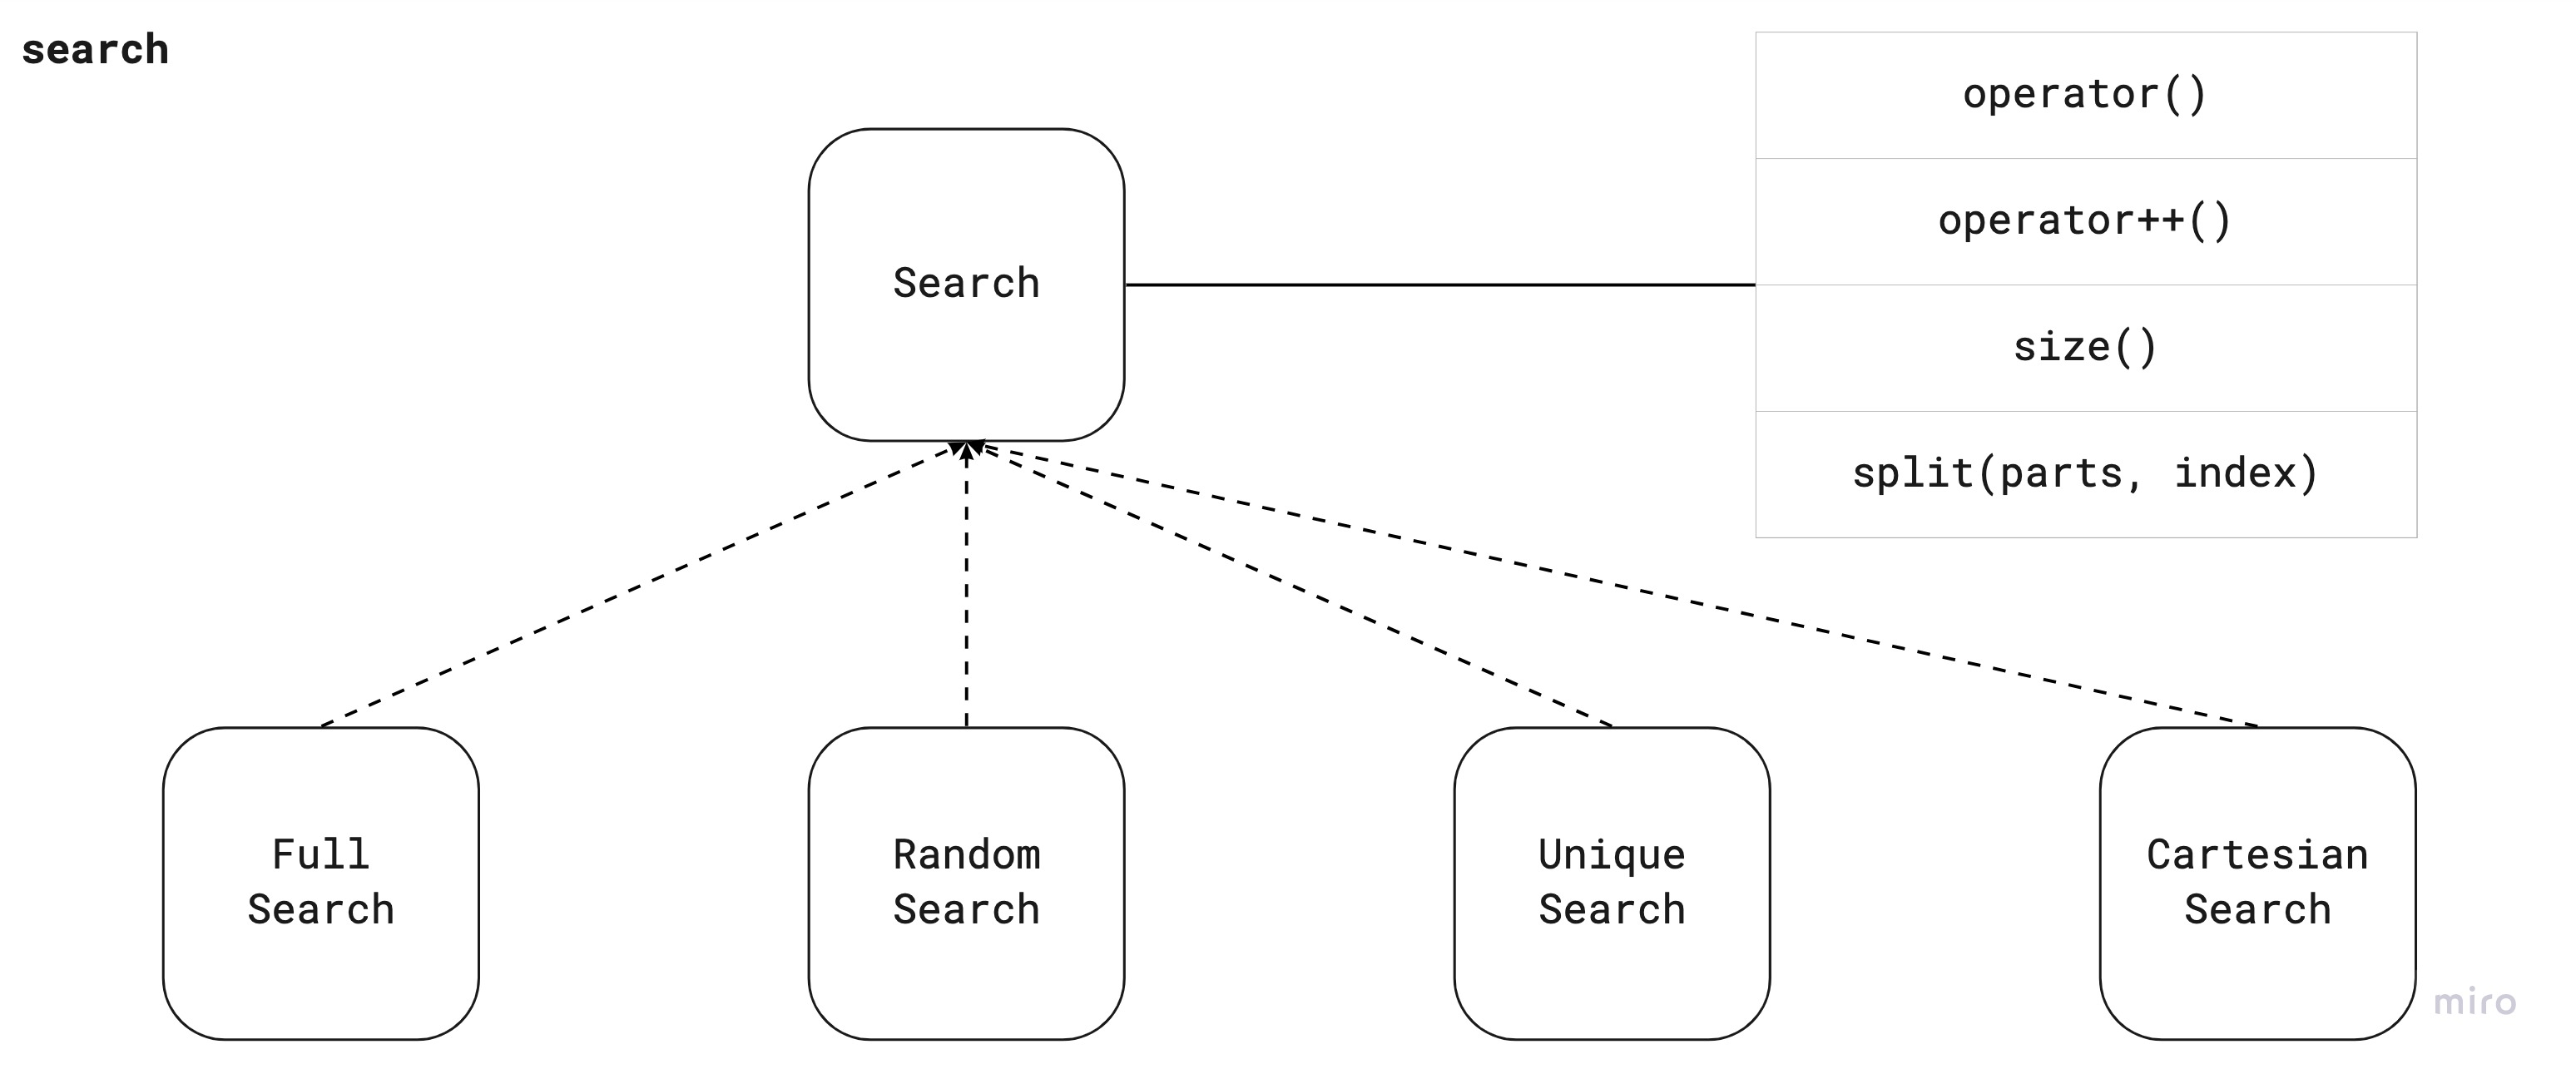
\includegraphics[width=\textwidth]{arch-search}
    \label{arch:rbs:prop:search-img}
\end{figure}

\begin{table}[H]
    \caption{Описание методов \textsc{Search}}\label{arch:rbs:prop:search-def}
    \centering
    \begin{tabularx}{\textwidth}{|*{3}{>{\centering\arraybackslash}X|}}\hline
        Метод & Параметры & Описание \\\hline
        \textsc{operator()} & -- & Возвращает текущий элемент выборки \\\hline
        \textsc{operator++} & -- & Переходит на следующий элемент выборки. Возвращает \textsc{false},
                                    если новый элемент -- последний \\\hline
        \textsc{size} & -- & Возвращает размер выборки \\\hline
        \textsc{split} & Число потоков, номер потока & Возвращает часть исходной выборки \\\hline
    \end{tabularx}
\end{table}

После получения выборки необходимо вызвать метод вывода последствий на всех элементах этой
выборки. Далее будут рассмотрены различные подходы к решению этой задачи: \textit{наивный
(последовательный), параллельный, вычисление $\rho$ через дерево поиска}.

\textit{Наивный подход}\label{arch:rbs:prop:naive}. Данный подход подразумевает последовательный
вызов метода вывода последствий. То есть, имея выборку $D$ и решатель $A$, значение $\rho$ 
аппроксимируется так, как показано в листинге \ref{arch:rbs:prop:naive-lst}.

\algdef{SE}[DOWHILE]{Do}{doWhile}{\algorithmicdo}[1]{\algorithmicwhile\ #1}%

\begin{algorithm}[H]
\caption{Наивное вычисление $\hat{\rho}$}\label{arch:rbs:prop:naive-lst}
\begin{algorithmic}
	\Function{calculate\_rho}{\textsc{A}, \textsc{D}}
        \State $S \leftarrow 0$
        \Do
            \State $\hat{b} \leftarrow \textsc{D()}$
            \If{\textsc{A($\hat{b}$)} = 0}
				\State $S \leftarrow S + 1$
			\EndIf
        \doWhile{\textsc{D++}}
        \State\Return $\frac{S}{N}$
	\EndFunction
\end{algorithmic}
\end{algorithm}

\textit{Параллельная обработка выборки}\label{arch:rbs:prop:par}. Данный подход разделяет выборку
на несколько выборок и обрабатывает их в разных потоках. Для этого используется метод \textsc{split}.
Псевдокод данного подхода представлен в листинге \ref{arch:rbs:prop:par-lst}.

\begin{algorithm}[H]
\caption{Параллельное вычисление $\hat{\rho}$}\label{arch:rbs:prop:par-lst}
\begin{algorithmic}
    \Function{calculate\_rho\_par}{$[\textsc{A}_i, i=\overline{1,M}]$, \textsc{D}}
        \State $S \leftarrow 0$
        \State $[\textsc{D}_i] \leftarrow \left[\textsc{D.split($M$, $j$),~ $j=\overline{1,M}$}\right]$
        \State\Return $\sum_{i}^{\textsc{parallel}}{\textsc{calculate\_rho($A_i$, $D_i$)}} / N$
	\EndFunction
\end{algorithmic}
\end{algorithm}

Данный подход с теоретической точки зрения крайне хорошо масштабируется, так как метод \textsc{split}
занимает несравнимо мало времени по сравнению с многократным вызовом метода вывода последствий. Практическое
сравнение последовательного и параллельного подходов приведено в разделе \ref{research:prop}.

\textit{Вычисление точного значения $\rho$ через дерево подстановок}\label{arch:rbs:prop:tree}.
Данный подход является новым и не имеет аналогов в известных мне решателях за ненадобностью. Однако,
идея, описанная далее, является крайне эффективной оптимизацией перебора $\hat{B}$, как показано в
разделе~\ref{research:prop}. Для вычисления точного значения $\rho$ необходимо посчитать число
подстановок $\hat{b} \in \hat{B}$, которые решаются заданным алгоритмом $A$. В данной работе, как
упомянуто ранее, в качестве этого алгоритма используется алгоритм вывода последствий. Результатом
работы этого алгоритма может быть либо информация о существовании конфликтующих подстановок переменных,
либо отсутствие дополнительной информации. Заметим, что если на каком-то префиксе $\hat{b}$ 
алгоритм сообщил о конфликте, то нет никакого смысла далее рассматривать подстановки с этим префиксом,
так как все они заведомо конфликтные. Можно просто прибавить к результату размер всего поддерева поиска.
Иллюстрация к данной идее приведена на рисунке \ref{arch:rbs:prop:tree-img}. Листинг, содержащий
псевдокод данного метода, приведен в приложении (листинг~\ref{append:rbs:prop:tree-lst}).
Отметим, что алгоритмы поиска вероятностных лазеек, описанные в разделе~\ref{arch:rbs:schema},
чья эффективность напрямую зависит от эффективности вычисления $\rho$, ищут лазейки, значение
$\rho$ которых достаточно быстро становится близким к единице. Это наблюдение дает основания
полагать, что производительность данного метода будет очень высокой, так как доминирующее
число поддеревьев будет отсечено на ранней стадии. Данный метод был успешно реализован и встроен 
в исходный код решателя Minisat. Сравнительные результаты с наивным и параллельным подходами 
содержатся в разделе~\ref{research:prop}.

\begin{figure}[H]
    \caption{Вычисление $\rho$ через дерево подстановок. Здесь $X,Y,Z$ --- переменные. Подстановки
    $E[X \mid 1]$ и $E[\{\,X,Y\,\} \mid \{\, X \to 0,~ Y \to 1 \,\}]$ приводят к конфликту, поэтому
    соответствующие поддеревья поиска можно не рассматривать.}
    \centering
    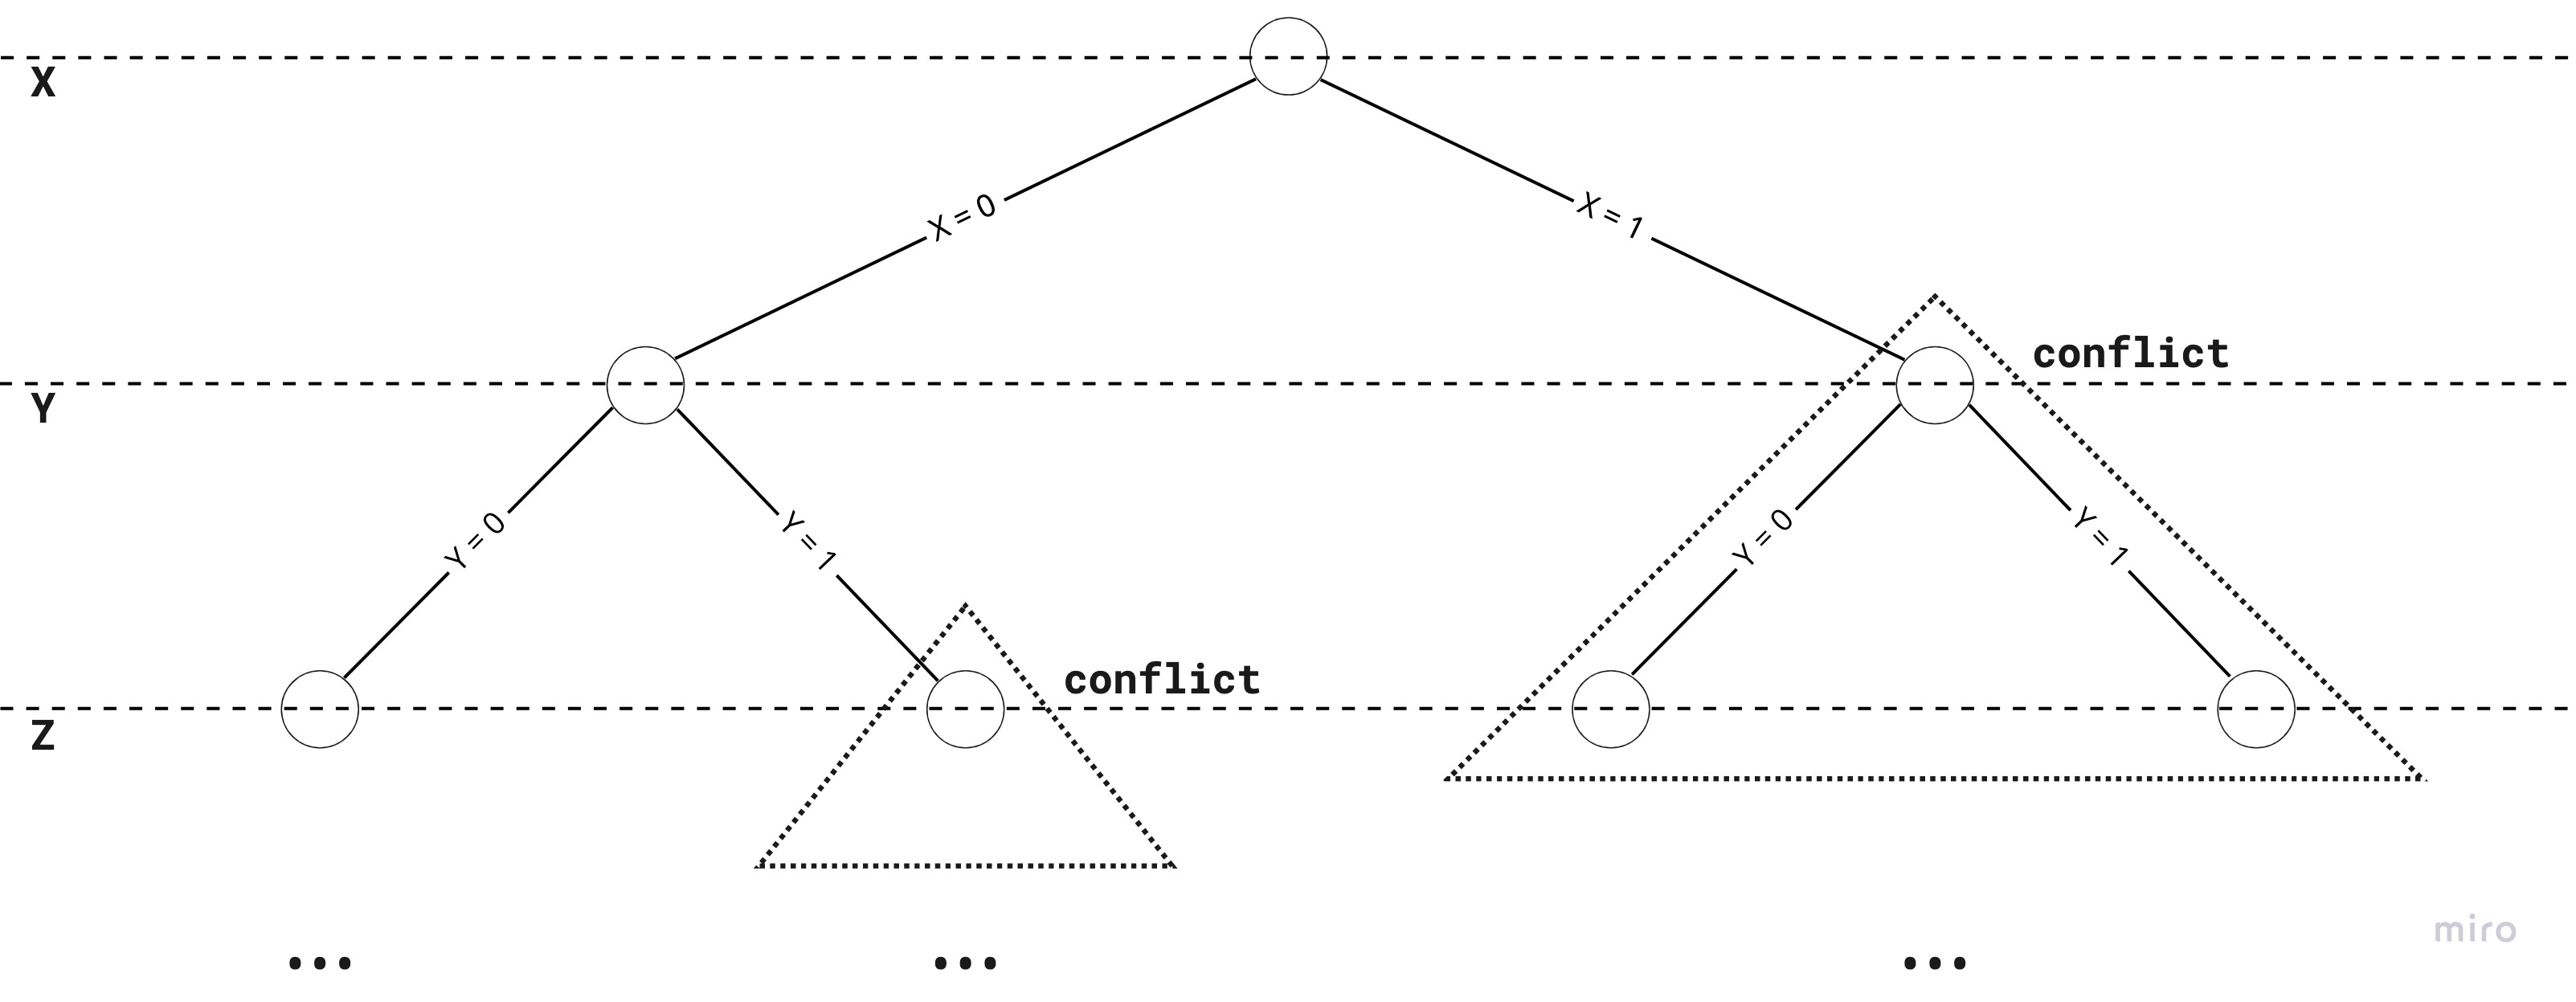
\includegraphics[width=\textwidth]{arch-tree}
    \label{arch:rbs:prop:tree-img}
\end{figure}

\section{Решение набора подстановок}\label{arch:solver}

В данном разделе описана архитектура сервиса решения булевой функции с подстановками. Описан интерфейс
сервиса, приведена схема распределения задач по последовательным решателям, описана техника обмена
знаниями между решателями.

В качестве последовательных решателей используются Minisat~\cite{bib:minisat},
MapleCOMSPS~\cite{bib:maplecomsps}, painless-maplecomsps~\cite{bib:painless}. Под последовательным
имеется в виду не тип самого решателя, а невозможность параллельного решения разных задач.
То есть, painless-mcomsps является параллельным решателем, но может решать лишь одну задачу
одновременно. Описываемый сервис нужен именно для того, чтобы обеспечить возможность параллельного 
решения разных задач, что необходимо для реализации параллельных алгоритмов решения на основе 
подхода разделяй-и-властвуй.

Схема наследования интерфейса \textsc{SolverService} проиллюстрирована на рисунке~\ref{arch:solver:serv-img}.
Описание методов интерфейса приведено в таблице~\ref{arch:solver:serv-def}.

\begin{figure}[H]
    \caption{Интерфейс \textsc{SolverService} и его реализация}
    \centering
    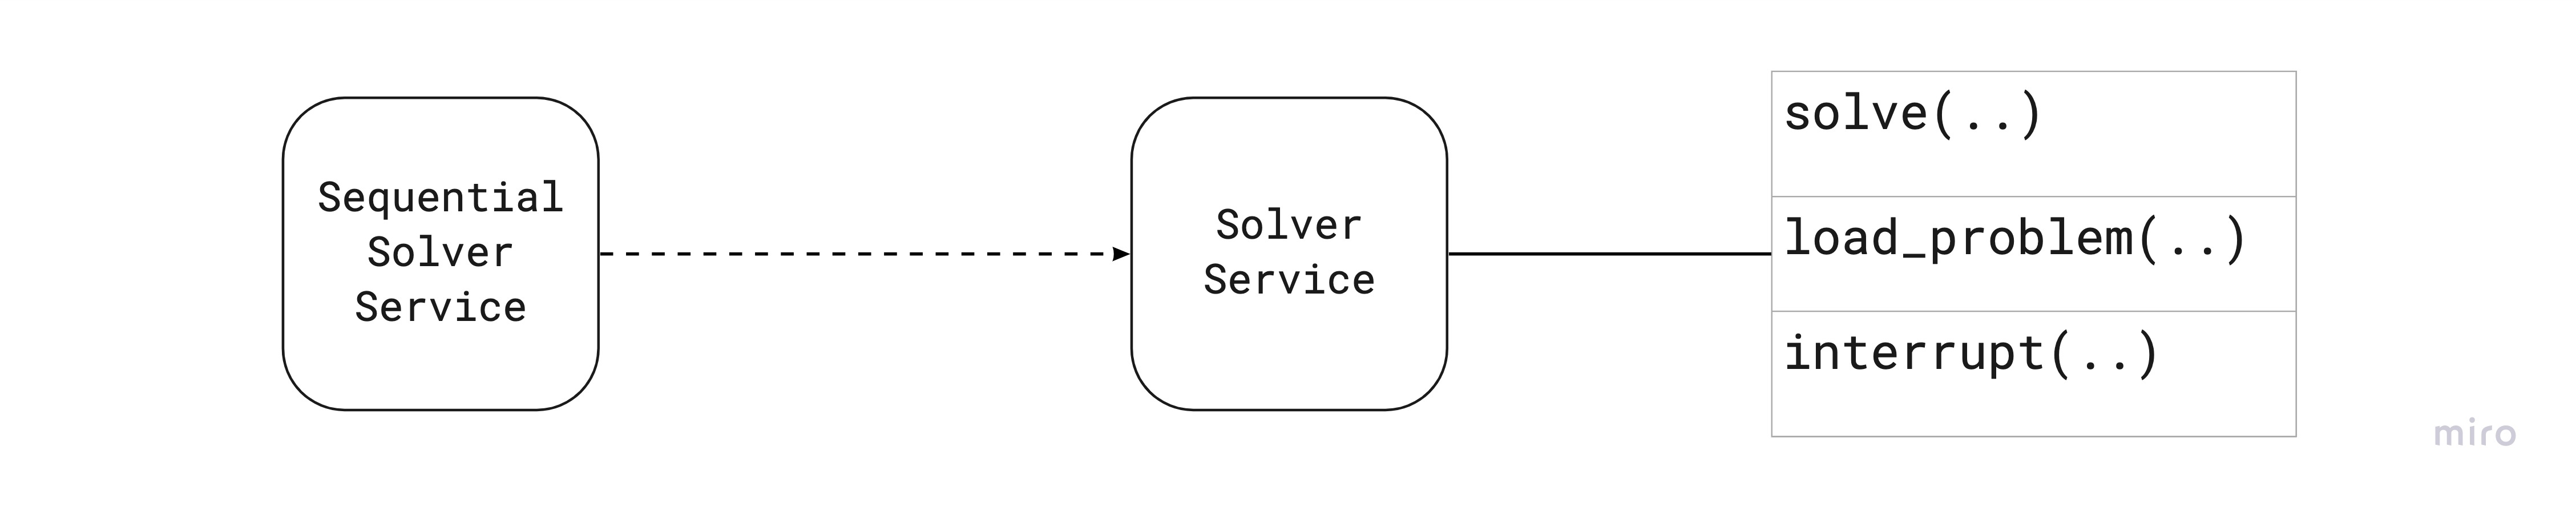
\includegraphics[width=\textwidth]{arch-solver}
    \label{arch:solver:serv-img}
\end{figure}

\begin{table}[H]
    \caption{Описание методов \textsc{SolverService}}\label{arch:solver:serv-def}
    \centering
    \begin{tabularx}{\textwidth}{|*{3}{>{\centering\arraybackslash}X|}}\hline
        Метод & Параметры & Описание \\\hline
        \textsc{solve} & Подстановка, ограничение по времени, callback-функция, вызываемая 
                        при окончании решения & Возвращает объект \textsc{std::future} типизированный
                        результатом решения, и добавляет задачу в очередь \\\hline
        \textsc{load\_problem} & -- & Загружает формулу в решатель \\\hline
        \textsc{interrupt} & -- & Прерывает процесс решения \\\hline
    \end{tabularx}
\end{table}

Реализация \textsc{SequentialSolverService} управляет набором последовательных решателей, работающих
параллельно: обеспечивает их задачами, а также, при необходимости, обеспечивает обмен знаниями.
Для распределения задач реализована безопасная для использования в многопоточной среде очередь.
Для обмена знаниями используются механизмы, реализованные в фреймворке 
\textsc{painless}~\cite{bib:painless-sharing} и адаптированные для использования разных решателей 
и схем обмена. Схема работы \textsc{SequentialSolverService} приведена на рисунке~\ref{arch:solver:seq-img}.

\begin{figure}[H]
    \caption{Схема работы \textsc{SequentialSolverService}}
    \centering
    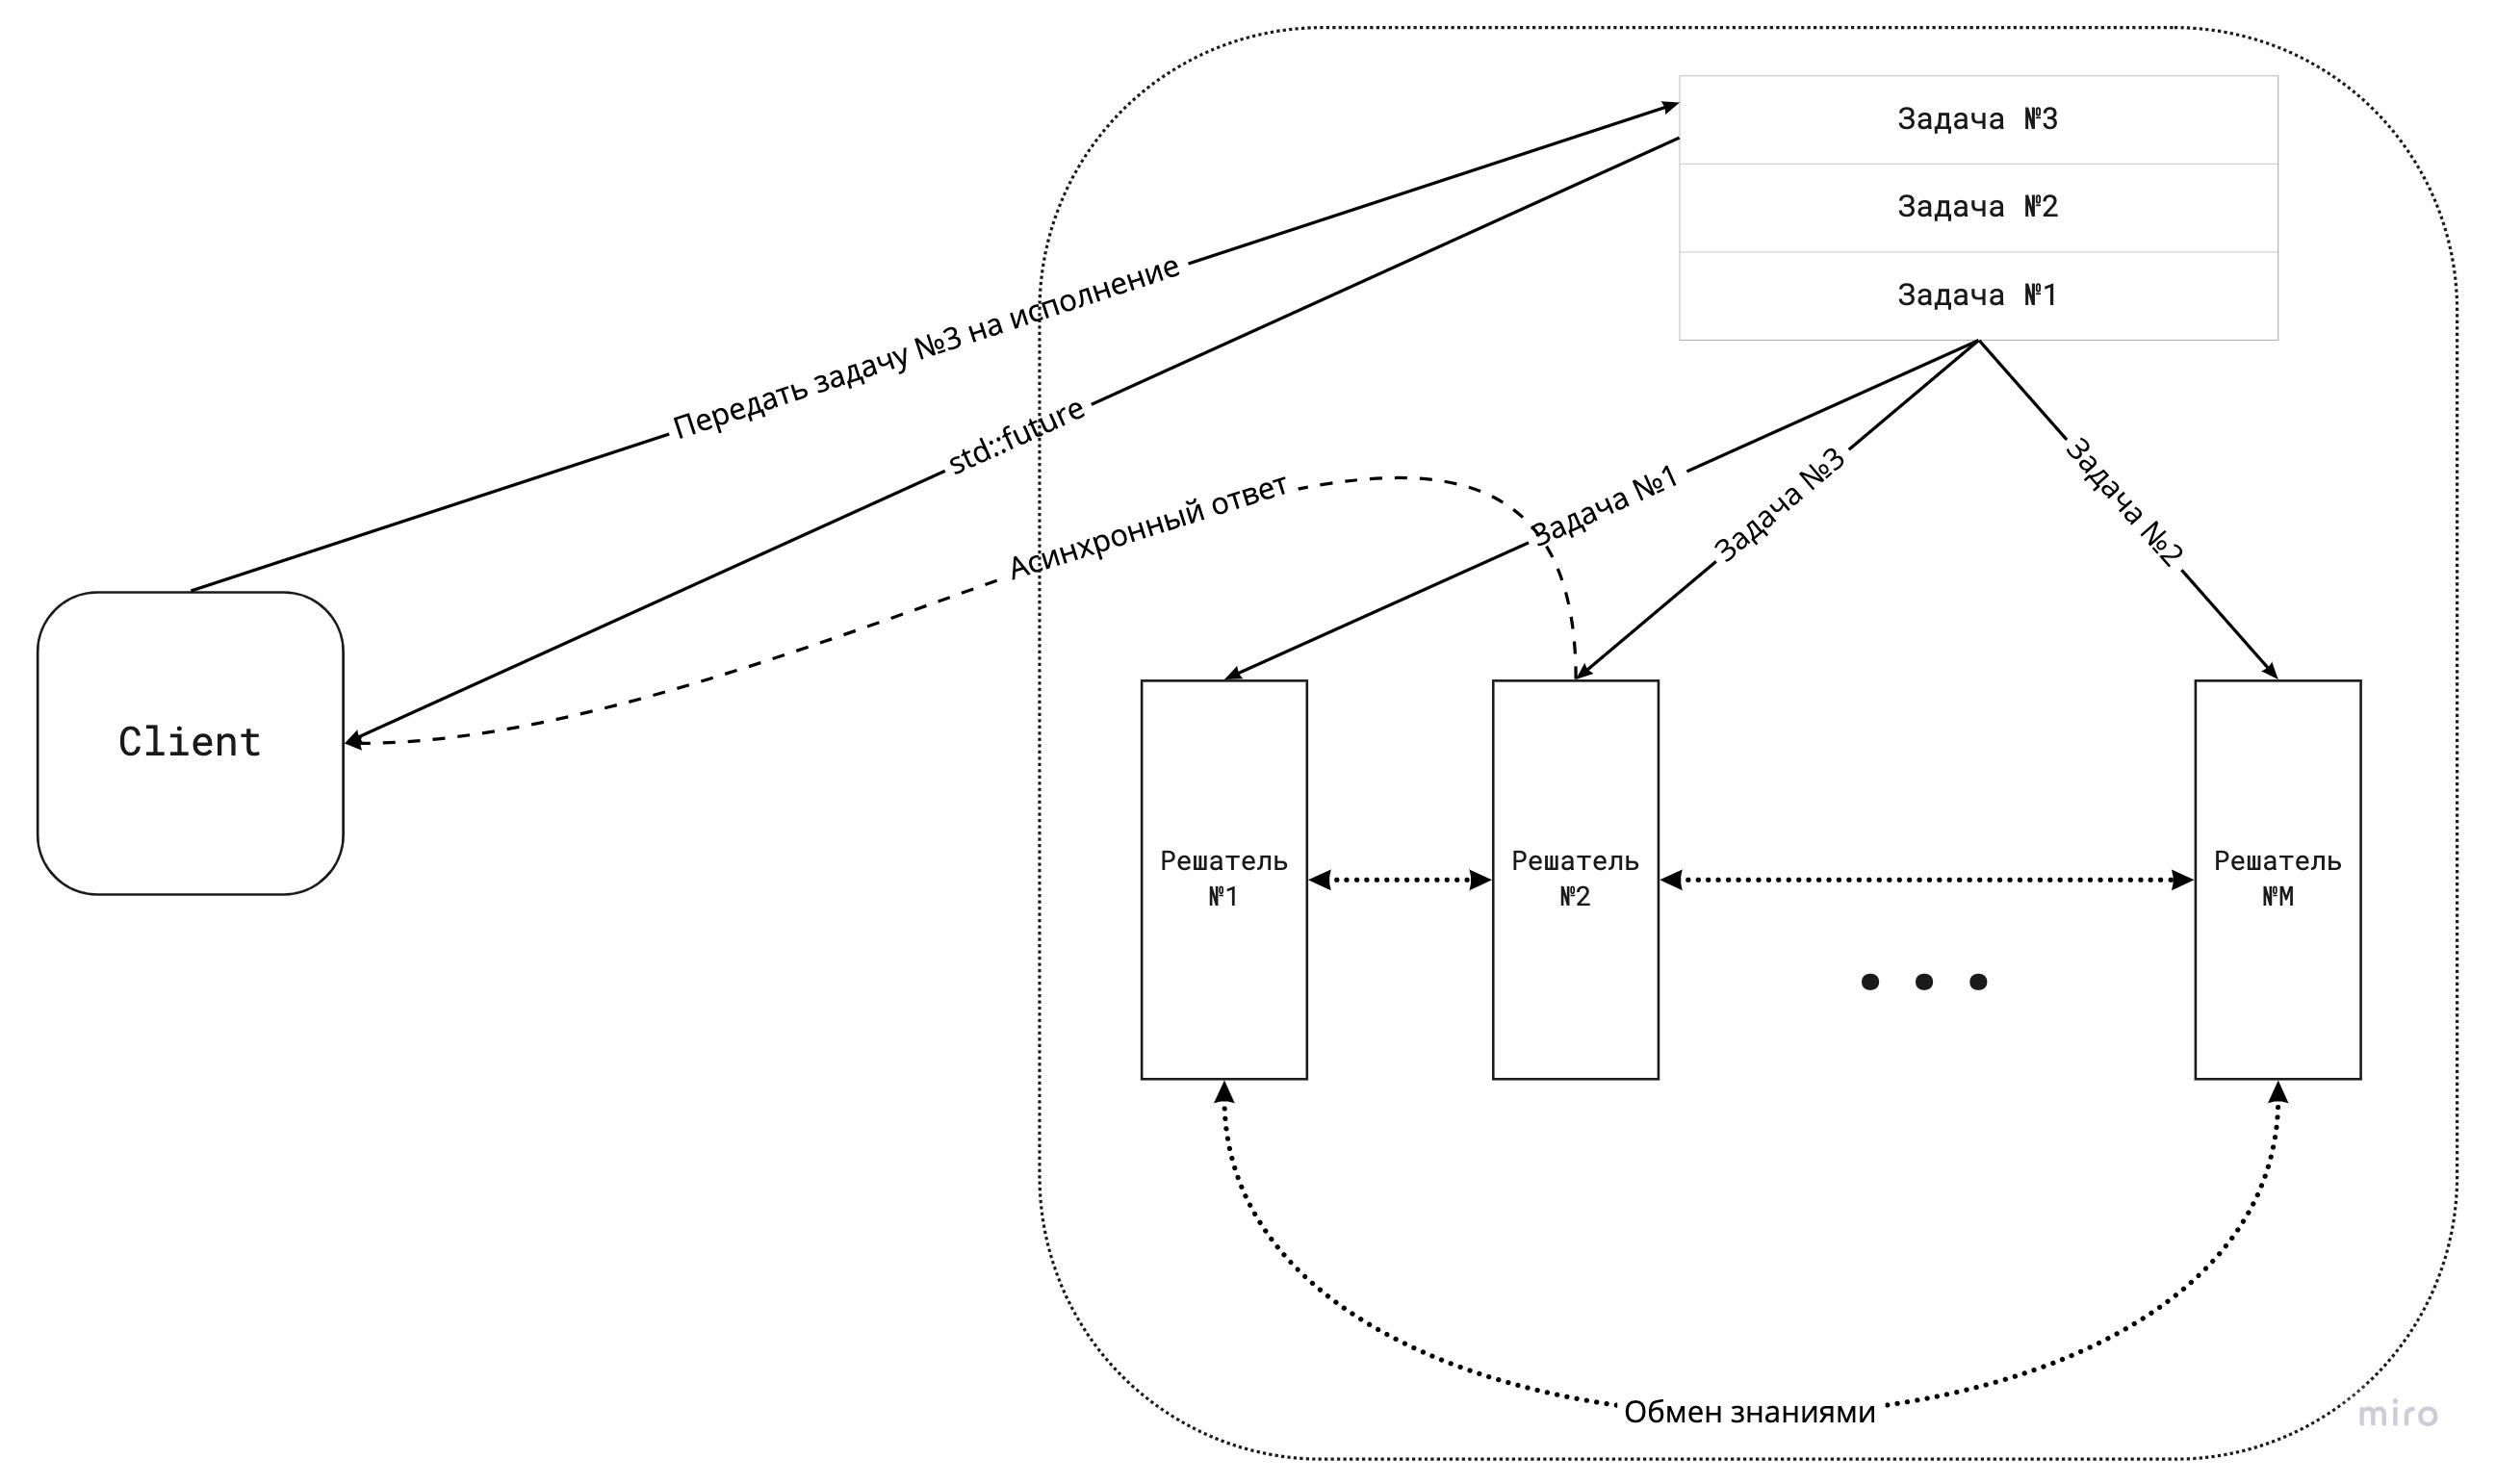
\includegraphics[width=\textwidth]{arch-seq}
    \label{arch:solver:seq-img}
\end{figure}

Как уже было упомянуто, для обмена знаниями используются алгоритмы в составе фреймворка \textsc{painless}~
\cite{bib:painless}. Также, решатель \textsc{painless-mcomsps} используюется в качестве одного из 
вариантов реализаций последовательных решателей. В связи с этим стоит отметить, что данный фреймворк 
по своей надежности и качеству кода не удовлетворяет требованиям, которые требуются для описываемого 
сервиса. А именно, в процессе исправления и рефакторинга кода фреймворка было устранено большое множество 
ошибок, как логических, так и програмных. Из критических проблем стоит отметить как минимум две:
\textsc{MapleCOMSPS}~\footnote{\url{https://github.com/vvallade/painless-sat-competition-2021/blob/b34579ca555a2989b610c3ac5df00711a76f2505/painless/mapleCOMSPS/mapleCOMSPS/core/Solver.cc#L1275}},
приводящую к некорректному поведению в ряде редких случаев, а также некорректную реализацию основного
метода класса \textsc{Reducer}~\footnote{\url{https://github.com/vvallade/painless-sat-competition-2021/blob/b34579ca555a2989b610c3ac5df00711a76f2505/painless/painless-src/solvers/Reducer.cpp#L149}},
приводящую к неустойчивости решателя к прерываниям.

\section{Описание реализации}\label{arch:impl}

\tbd{Надо ли это вообще?}
В данном разделе описана структура исходного кода программы, перечислены возможные опции как при
сборке, так и при запуске приложения.

\chapterconclusion

\tbd{Заключение}
